Для разработки процессорной системы существует возможность использовать готовые блоки, предоставляемые компанией - производителем Xilinx. В данной работе используются некоторые из них. Также для передачи комманд и параметров оператора был разработан пользовательский блок виртуальных регистров. Список всех блоков и их краткое описание представлены в таблице()\par
\begin{table}
    \caption{Блоки дизайна процессорной системы}
    \begin{tabular}{|>{\centering\arraybackslash}p{0.5\textwidth}|>{\centering\arraybackslash}p{0.5\textwidth}|}
        \hline
        Наименование блока & Описание \\
        \hline
        Процессорная система ZYNQ7 & Программный интерфейс вокруг процессорной системы платформы Zynq-7000 \\
        \hline
    \end{tabular}
\end{table}
На рисунке() представлена диаграмма блоков процессорной системы.\par
\begin{figure}[ht]
    \centering
    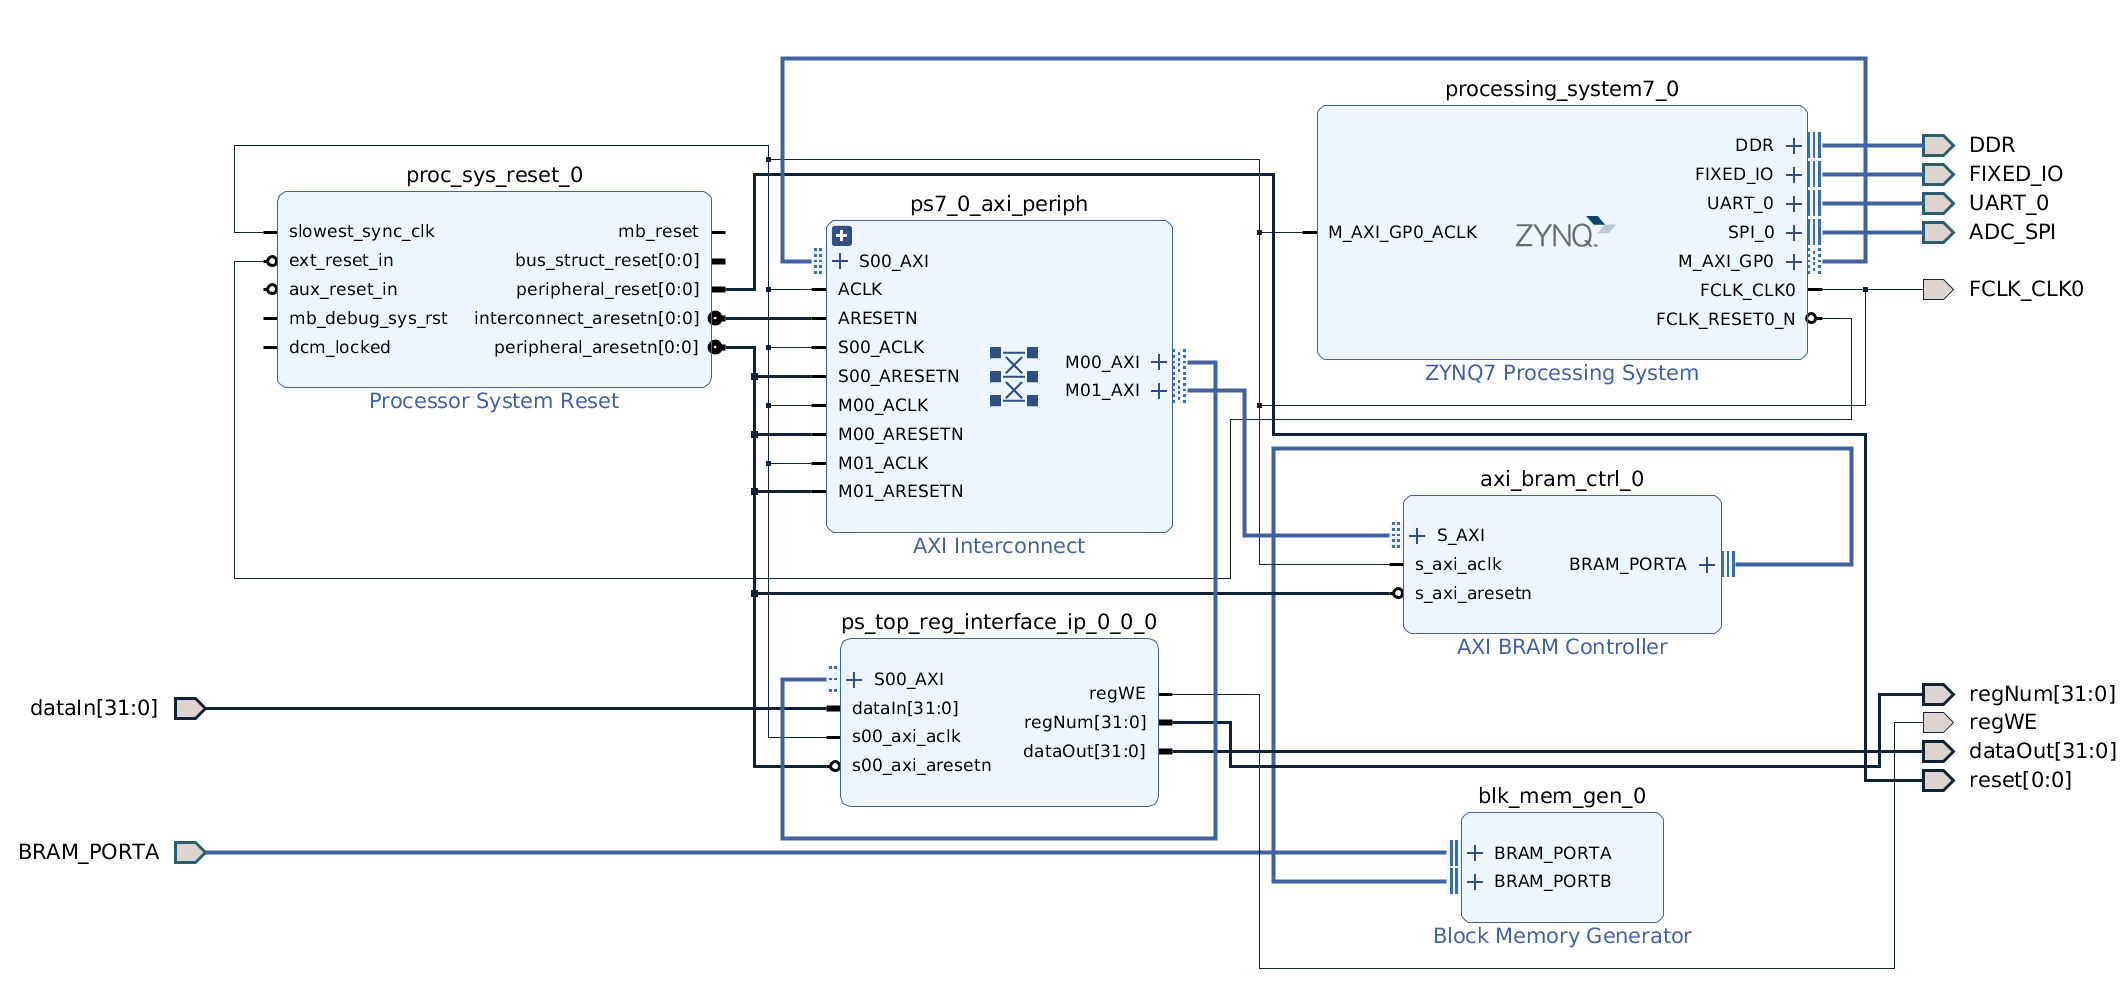
\includegraphics[width=1\linewidth]{ps_top.jpg}
    \caption{Диаграмма блоков процессорной системы}
    \label{fig:mpr}
\end{figure}
